\chapter{Production Theory}

Production theory parallels consumer theory, with firms in place of
consumers and profit in place of utility. We will build the firm's
problem in stages: first describe what the firm \emph{can} do (the
production set), then ask what the firm \emph{wants} (profit
maximization or, when output is given, cost minimization).

\section{Setups}\label{setups-2}

We begin with the standard assumptions that justify treating the firm
as a profit-maximizer in a competitive market.
\asm{}{
\begin{enumerate}
\item
  \textit{Perfect/complete} information: no uncertainty about input/output
  prices, production technology, etc.
\item
  \textit{Perfectly competitive} input and output markets: firms are price-takers
  in both input and output markets.
\item
  Input/output prices are \textit{linear}, justified by perfectly competitive
  markets.
\item
  Goods are perfectly \textit{divisible}.
\item
  The technology is \textit{exogenously given}.
\item
  The firm's managers are \textit{perfectly controlled by the
  owners/shareholders.}
\end{enumerate}
}

\rmkb{
\begin{enumerate}

\item
  Assumptions 1, 2, and 6 are what make ``maximize profit'' an
  unambiguous objective. Drop any of them and the objective itself
  becomes contestable:

  \begin{itemize}
  \item
    Drop 1 (perfect information): owners with different risk
    preferences will disagree about which uncertain profit stream to
    maximize.
  \item
    Drop 2 (price-taking): an owner who also has market power on the
    input or output side may prefer outcomes that distort the firm away
    from profit maximization.
  \item
    Drop 6 (perfect alignment): managers may pursue their own
    objectives — the agency problem.
  \end{itemize}
\item
  Why is profit maximization determined by assumption 6 specifically?
  Consider a firm jointly owned by \(I\) consumers, with consumer \(i\)
  holding share \(\theta_i\ge 0\) and \(\sum_i \theta_i = 1\). Consumer
  \(i\)'s utility maximization problem is
  $$
\begin{aligned}
  & \max_{\x_i\ge \0} u_i(\x_i)\\
  \text{s.t. }& \p\cdot \x_i\le m_i + \theta_i \p\cdot\y
  \end{aligned}
$$

  Under local non-satiation, \(v(\p,m)\) is strictly increasing in
  \(m\). Every shareholder therefore strictly prefers higher
  \(\p\cdot\y\) — the firm's profit — regardless of how heterogeneous
  their preferences over consumption bundles are. The unanimous
  shareholder objective is profit maximization. Drop assumption 6
  (perfect manager-owner alignment) and managers might not implement
  this objective.
\end{enumerate}
}

\subsection{Production Set}\label{production-set}

\defn{Production Plan; Production Set}{
A \textit{production plan} is a vector \(\y = (y_1,y_2,\cdots,y_n)\in \RR^n\), where \(y_i\) can be either positive or negative, with
\(y_i>0\) standing for an output and \(y_i<0\) an input.

The \textit{production set} of a firm is described by \(Y\subset \RR^n\), where
any \(\y\in Y\) is a \emph{feasible} production plan, i.e., a
production plan the firm can choose from.
}

\ex{
For example, consider the example of one input and one output, suppose
the production set is given by \(Y = \{(-L,y): y \le f(L),L\ge 0 \}\),
where \(f(\cdot)\) is the production function. The production set \(Y\)
is the gray-shaded area:
\begin{center}
    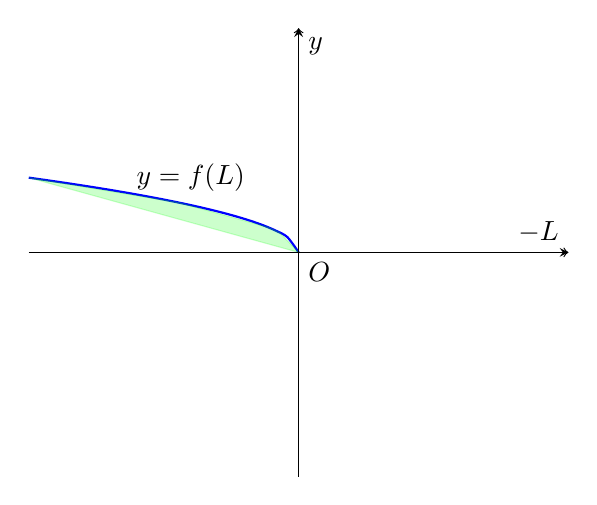
\begin{tikzpicture}
    \begin{axis}[
        xmin=-9, xmax=9, 
        ymin=-9, ymax=9, 
        axis lines=center,
        xlabel={$-L$},
        ylabel={$y$},
        xtick=\empty,
        ytick=\empty,
        axis on top,
        clip=false, 
        legend style={at={(0.5,-0.2)},anchor=north} 
    ]

    \addplot[domain=-9:0, smooth, no markers, blue, thick] {sqrt(-x)};

    \node[below right] at (axis cs:0,0) {$O$};


     \addplot [green,fill=green,opacity=0.2,
    ] coordinates {
        (-9,3) (-4,2) (-1,1) (-0.64,0.8) (0,0)
    }
        |- (0,0) -- cycle;

    \draw[->] (axis cs:-9,0) -- (axis cs:9,0);
    \draw[->] (axis cs:0,-9) -- (axis cs:0,9);

    \node[anchor=center] at (axis cs:-3.6,3) {$y = f(L)$};
    
    \end{axis}
\end{tikzpicture}
\end{center}
}

Throughout our analysis, we will make the innocent technical assumptions
that \(Y\) is \textit{non-empty} (so as to have something to study),
\emph{closed} (to help ensure the existence of optimal production
plans), and \(Y\ne \RR^n\) (so that there is some scarcity). In addition to those, some other assumptions are needed to make the problem more practical.

\asm{Production Set}{
\begin{enumerate}
\item
  \(Y\ne \varnothing\).
\item
  {\(Y\) is \textit{closed}}.
\item
  {\textit{No free lunch} and the possibility of \textit{shutdown}}:
  \(Y\cap \RR_+^n = \{\0\}\).
\item
  \textit{Free disposal}: \(\y\in Y \too \y'\in Y\), for any \(\y'\le \y\).
\end{enumerate}
}

\rmkb{
Recall the distinction between the short run and the
long run from intermediate microeconomics:

\begin{itemize}
\item
  Short run: some inputs are fixed.
\item
  Long run: all inputs are variable.
\end{itemize}

In our discussion, we will mostly focus on the \textbf{long run} in
advanced microeconomics. That is, all inputs are by default changeable.
}

\subsection{Firm's Profit Maximization Problem}\label{firms-profit-maximization-problem}

In the spirit of rational decision-making, the firm's
problem can be framed as choosing the profit-maximizing production plan
from its production set.

\defn{Profit Maximization Problem}{
$$
\begin{aligned}
& \max_{\y} \p\cdot\y \\
\text{ s.t. } & \y\in Y
\end{aligned}
$$
}

Similarly, we define the firm's profit function and optimal supply correspondence, following the same logic with consumer theory.

\defn{Profit Function}{
\textit{Profit function} is defined as the optimal value function of the firm's profit given $\p$:
\[\pi(\p) = \sup_{y\in Y} \p\cdot\y.\]
}

\defn{Optimal Supply Correspondence}{
\textit{Optimal supply correspondence} is defined as the firm's optimal choice(s) given $\p$:
\[\y^*(\p) = \arg \max_{\y\in Y} \p\cdot\y = \{\y\in Y: \p\cdot\y = \pi(\p) \}.\]
}

\rmkb{
\begin{itemize}
\item
  We have not made sufficient assumptions to ensure that a maximum
  profit is achieved (i.e., \(y^*(\p)\ne\varnothing\)), so the \(\sup\) in
  profit function cannot always be replaced with the \(\max\).

  \ex{
  A firm uses labor
  and capital to produce its sole output. The production function is
  given by \(f(L,K) = \sqrt{LK}\). Suppose \(p = 4\) and \(w = r = 1\). If the firm chooses \(L= K =t\), the profit is given
  by \(\pi = 2t\), which is unbounded in \(t\).
  }
\item
  \(y^*(\p)\), the optimal supply correspondence, is a set-valued
  function, which maps an element from one set, the domain of the
  function, to a subset of another set.
\end{itemize}
}

\section{Profit Maximization and Rationalizability}\label{profit-maximization-and-rationalizability-2}

The firm's analog of consumer theory's central questions is:

\begin{enumerate}
\item
  Given (some of) the firm's supply decisions \(y(\p)\) — but \emph{not}
  the production set \(Y\) — when is \(y(\cdot)\) consistent with
  profit maximization for some production set? (Rationalizability.)
\item
  When does the firm's profit maximization problem have a solution?
\item
  What properties do the profit function \(\pi(\cdot)\) and the optimal
  supply correspondence \(y^*(\cdot)\) inherit from the setup?
\item
  How do we actually solve the firm's problem?
\end{enumerate}

These mirror the revealed-preference questions for consumers, but with
the inference direction reversed. In consumer revealed preference we
observe the feasible set and try to recover the objective; here we
observe the objective (profits at various prices) and try to recover
the feasible set (the production set).

In practice, we do not know a firm's production set
\(Y\), but observe some of its supply choice \(y(\p)\) for
\(\p\in \RR^n\). Hence, we define rationalizability on empirical
meanings.

\defn{Rationalizability}{
Empirical supply correspondence
\(y:\RR^n \rightrightarrows \RR^n\) is \textit{rationalized} by production set
\(Y\) if \(y(\p)\subset y^*(\p) = \arg\max_{\y\in Y} \p\cdot\y\) for all
\(\p\in \RR^n\). Empirical supply correspondence \(y(\cdot)\) is
\textit{rationalizable} if it is rationalized by some production set.
}

Intuitively, an observed supply correspondence \(y(\cdot)\) is
  rationalizable if we can find a production set \(Y\) such that
  \(y(\cdot)\) is consistent with rational decision-making.

\rmkb{
\begin{itemize}
\item
  We may only observe some of the optimal choice(s) at each price
  \(\p\), so in the definition it writes ``\(y(\p)\subset y^*(\p)\)".
\item
  Practically, it is not necessary that we observe all of the firm's
  optimal supply decisions at all prices. We can define without loss that 
  \(y(\p_0) = \varnothing\) if the firm's supply decision is not observed at
  \(\p_0\).
\end{itemize}
}

We are naturally interested in what we can infer about the production set \(Y\) from the empirical observations if the supply choices are rationalizable. Suppose at price \(\p\) the firm chooses production plan \(y(\p)\).
Here are two plausible inferences:

\begin{enumerate}
\item
  Plan \(y(\p)\) must be feasible, i.e., \(y(\p)\in Y\).
\item
  Any production plan \(\y\) other than elements in \(\y(\p)\) must
  generate no more profits than elements in \(y(\p)\) at price \(\p\).
  Or equivalently, any production plan \(\y\) that is more profitable
  than \(\y(\p)\) at price \(\p\) cannot be feasible.
\end{enumerate}

We use the first idea to construct an ``inner bound" on \(Y\) defined by all choices that the firm has actually made, as they must first be feasible to be chosen. We use the
second idea to construct an ``outer bound" on \(Y\), which only includes
plans that do not give the firm greater profits than its observed choices at any given price \(\p\).

\defn{Inner Bound; Outer Bound}{
Given empirical supply correspondence \(y(\cdot)\),
we define the \emph{inner bound} of the firm's
production set as:
\[Y^I = \bigcup _{\p\in \RR^n}y(\p),\]
\hspace{2em} and the \emph{outer bound} of the firm's production set
as:
\[Y^O = \{\y\in \RR^n: \p\cdot\y\le \p\cdot\y_{\p}, \forall \p\in\RR^n \text{ and }\y_{\p}\in y(\p) \}.\]
}

Intuitively, any optimal supply choice(s) must be feasible, so
\(Y^I\subset Y\); and any feasible production plan cannot yield a
strictly higher profit at any price, so \(Y\subset Y^O\). This intuition is formally characterized in the following proposition.

\propp{Rationalizable Empirical Supply Correspondence}{
Production set \(Y\) rationalizes empirical supply
correspondence \(y(\cdot)\) if and only if
\[Y^I\subset Y\subset Y^O.\]
}{
\begin{enumerate}
\item
  ``Only if"

  \begin{itemize}
  \item
    First consider any \(\z\in Y^I\). By definition of \(Y^I\),
    there exists a \(\p\) such that \(\z\in y(\p)\). Since \(y(\cdot)\)
    is rationalizable, \(y(\p)\subset y^*(\p)\subset Y\). It follows
    that \(\z\in Y\) and \(Y^I\subset Y\).
  \item
    Next consider any \(\y\in Y\) and \(\p\in \RR^n\). Since \(y(\cdot)\)
    is rationalizable, \(y(\p)\subset y^*(\p)\). By the definition of
    \(y^*(\p)\), for any \(\y_{\p}\in y^*(\p)\),
    \(\p\cdot\y\le \p\cdot \y_{\p}\). It follows that \(\y\in Y^O\) and
    \(Y\subset Y^O\).
  \end{itemize}
\item
  ``If"

  \begin{itemize}
  \item
    Fix \(\p\in \RR^n\) and consider any \(\y_{\p}\in y(\p)\).
  \item
    Since \(y(\p)\subset Y^I\subset Y\), \(\y_{\p}\in Y\).
  \item
    Moreover, for any \(\y\in Y\subset Y^O\),
    \(\p\cdot\y\le \p\cdot\y_{\p}\). Consequently,
    \(\y_{\p}\in y^*(\p)\).
  \end{itemize}
\end{enumerate}
}

\rmkb{
For the ``if" part, by definition of \(Y^O\), if we fix any
\(\p\in\RR^n\), and take \(\y_{\p}\in y(\p)\), \(\y_{\p}\) maximizes
\(\p\cdot \y_{\p}\). However, with this condition we cannot simply
conclude that \(y(\cdot)\) is rationalizable, because $y_{\p}$ has to be in the production set $Y$, though it sounds trivial; or equivalently speaking, \(\y_{\p}\in Y^I\) may not fall in the outer bound \(Y^O\).
}

The proposition indicates that, \(Y^I\) and \(Y^O\) carry all the
information we have about the production set based on rational
decision-making. The proposition immediately implies the following two
corollaries:

\cor{Weak Axiom of Profit Maximization (WAPM)}{
Let
\(P = \{\p\in\RR^n: y(\p)\ne\varnothing \}\). Empirical supply correspondence
\(y(\cdot)\) is rationalizable if and only if \(Y^I\subset Y^O\), that
is, \(\p\cdot\y_{\p}\ge \p\cdot\y_{\p'}\), for any \(\p\in P\) and
\(\y_{\p}\in y(\p)\), \(\y_{\p'}\in y(\p')\).
}


One simple consequence of this characterization is that, when checking
rationalizability, we can restrict attention to supply functions rather
than correspondences. (Simply put, compared with the preceding
proposition, the production set \(Y\) is ``left out" here.)

WAPM directly implies ``law of supply".

\corp{Law of Supply}{
Suppose empirical supply
correspondence \(y(\cdot)\) is rationalizable and let
\(P = \{\p\in\RR^n:y(\p)\ne\varnothing \}\). Then for any \(\p\in P\) and
\(\y_{\p}\in y(\p)\), \(\y_{\p'}\in y(\p')\),
\[(\p-\p')\cdot (\y_{\p}-\y_{\p'})\ge 0.\]
}{
Since \(y(\cdot)\) is rationalizable, by WAPM, we have
\[\p\cdot \y_{\p}\ge \p\cdot \y_{\p'}.\]

Switching the role of \(\p\) and \(\p'\), we have
\[\p'\cdot \y_{\p'} \ge \p'\cdot \y_{\p}\]

Adding the two equations above, we get the ``law of supply".
}

In particular, if there is a single output and \(y(\cdot)\) is
single-valued, then
\[(p-p')(y(p)-y(p'))\ge 0\]

In other words, any rationalizable supply function must be
\textbf{(weakly) upward sloping}.

\cor{}{
Let \(P = \{\p\in\RR^n:y(\p)\ne\varnothing \}\).
Empirical supply correspondence \(y(\cdot)\) is rationalizable if and
only if:

\begin{enumerate}
\item
  Any selection \(\hat y:P\to \RR^n\) is rationalizable.
\item
  For any two selections \(\hat y\) and \(\tilde y\) and any
  \(\p\in P\), \(\p\cdot\hat y(\p) = \p\cdot \tilde y(\p)\). (Or
  equivalently, \(\pi(\p)\) is single-valued for each \(\p\in P\).)
\end{enumerate}
}

\rmkb{
\begin{itemize}
\item
  The first statement of this corollary is equivalent to WAPM applied to
  \(\p'\ne \p\),
\item
  The second statement of this corollary is equivalent to WAPM applied
  to \(\p' = \p\).
\item
  Thus, when given a supply correspondence, we only need to check that

  \begin{enumerate}
  \item
    Each selection from it is a rationalizable supply function, and
  \item
    The profit function \(\pi(\p) = \p\cdot \y\) is single-valued at any
    given \(\p\in P\); or equivalently speaking, \(\pi(\p)\) does not
    depend on which selection is chosen.
  \end{enumerate}

  Since checking the second condition is trivial, we can focus on
  rationalizability of supply functions (single-valued correspondence).
\end{itemize}
}

Verifying rationalizability by checking all the WAPM inequalities is
difficult when the set of observations is large. Fortunately, it turns
out that when we have a continuum of observations, rationalizability can
be verified much more easily using differential conditions.
Specifically, we now suppose that we observe the firm's
supply choices on an open convex set \(P\) of prices (e.g., \(P\) could
be the set of all strictly positive price vectors).

\propp{Rationalizability: Differentiable Case}{
Consider an empirical supply correspondence \(y(\cdot)\) whose domain
\(P = \{\p\in\RR^n:y(\p)\ne\varnothing \}\) is an open convex set. Suppose
that \(\pi(\p) = \p\cdot y(\p)\) is a differentiable function on
\(\p\in P\). Then \(y(\cdot)\) is rationalizable if and only if:

\begin{enumerate}
\item
  (\textbf{Hotelling's Lemma}) \(\nabla \pi(\p) = \y_{\p}\), for
  any \(\p\in P\) and \(\y_{\p}\in y(\p)\).
\item
  \(\pi(\cdot)\) is a convex function.
\end{enumerate}
}{
\begin{enumerate}
\item
  ``If"

  \begin{itemize}
  \item
    Fix \(\q\in P\) and take any \(\y_{\q}\in y(\q)\). Consider the
    ``difference function": \(G(\q;\p) = \p\cdot\y_{\q}-\pi(\p)\).
  \item
    It suffices to show that, \(G(\q;\cdot)\) is maximized at
    \(\p = \q\).
  \item
    Since \(\pi(\cdot)\) is a convex function, then \(G(\q;\cdot)\) is a
    concave function. Since \(G(\q;\cdot)\) is differentiable in \(\p\),
    the first-order condition is both necessary and sufficient.
  \item
    The F.O.C.: \(\y_{\q} - \nabla \pi(\p)|_{\p=\q} =0\), which is
    precisely the Hotelling's Lemma.
  \end{itemize}
\item
  ``Only if"

  \begin{itemize}
  \item
    The proof above also shows WAPM implies the
    Hotelling's lemma. Indeed, it is just an application
    of envelope formula. It remains to show \(\pi(\cdot)\) is a convex
    function.
  \item
    By rationalizability, there exists \(Y\) such that
    \(\pi(\p) = \sup_{\y\in Y} \p\cdot\y\).
  \item
    Take any \(\p,\q\in P\) and \(t\in (0,1)\). If \(\pi(\p) = +\infty\)
    or \(\pi(\q) = +\infty\), then clearly
    \(\pi(t\p + (1-t)\q)\le t\pi(\p)+ (1-t)\pi(\q)\). Otherwise,
    $$
\begin{aligned}
    \pi(t\p + (1-t)\q) = & \sup_{\y\in Y} (t\p + (1-t)\q)\cdot \y\\
     \le & t\cdot \sup_{\y\in Y}\p\cdot \y + (1-t)\cdot \sup_{\y\in Y}\q\cdot \y\\
     = & t\pi(\p)+ (1-t)\pi(\q)
    \end{aligned}
$$
  \end{itemize}
\end{enumerate}
}

\propp{Rationalizability: General Case}{
Consider
an empirical supply function \(y:P\to \RR^n\), where \(P\subset \RR^n\) is
a convex set. \(y(\cdot)\) is rationalizable if and only if:

\begin{enumerate}
\item
  (\textbf{Producer Surplus Formula}): \(\pi(\p) = \p\cdot y(\p)\) satisfies, for
  any smooth path \(\rho:[0,1]\to P\), with \(\rho (0) = \p\) and
  \(\rho(1) = \p'\),
  \[\pi(\p') - \pi(\p) = \int_0^1 y(\rho(t))\cdot \rho'(t)\text{d}t.\]
\item
  (\textbf{Law of Supply}): For \(\p,\p'\in P\),
  \[(\p-\p')\cdot (y(\p)-y(\p'))\ge 0.\]
\end{enumerate}
}{
\begin{itemize}
\item
  ``Only if" part

  We have already shown the ``law of supply", so it suffices to show the
  ``producer surplus formula".

  Let \(\phi(t) = \pi(\rho(t))\). Consider the ``difference function":
  $$
\begin{aligned}
  \delta(\theta;t) :=&  \rho(t)\cdot y(\rho(\theta)) - \pi(\rho(t)) \\
  =&  \rho(t)\cdot y(\rho(\theta)) - \phi(t)\\
  \end{aligned}
$$

  By rationalizability of \(y(\cdot)\),
  $$
\begin{aligned}
  & \delta(\theta;t) \le 0 = \delta (\theta;\theta)\\
  \too & \frac{\partial \delta(\theta;t)}{\partial t}\bigg|_{t = \theta} =0\\
  \iff&  \frac{\partial \delta(\theta;t)}{\partial t}\bigg|_{t = \theta} =y(\rho(\theta))\cdot \rho'(\theta)-\phi'(\theta) = 0\\
  \iff &\phi '(\theta) = y(\rho(\theta))\cdot \rho'(\theta)\\
  \too & \phi(1) - \phi(0) = \int_0^1 y(\rho(t))\cdot \rho'(t) \text{d}t\\
  \too & \pi(\p') - \pi(\p) = \int_0^1 y(\rho(t))\cdot \rho'(t) \text{d}t
  \end{aligned}
$$

  \rmk{
  In fact in order to derive the integral result from
  the derivatives, we have to prove the continuity of \(\phi(\cdot)\).
  It can be shown that \(\phi(\cdot)\) is Lipschitz continuous and hence
  absolutely continuous. The proof is rather technical and thus omitted here.
  }
\item
  ``If" part

  In order to show the rationalizability of \(y(\cdot)\), it suffices to
  show WAPM. Because the path integral is path-independent, take a straight line for math convenience:
  \[\rho(t) = \p+t(\p'-\p).\]

    We aim to prove
  \[\pi(\p') - \p'\cdot y(\p)\ge 0.\]

  Making tweaks to the difference in profit:
  $$
\begin{aligned}
  \pi(\p')-\p'\cdot y(\p) & = \pi(\p')-\pi(\p) + \pi(\p)-\p'\cdot y(\p)\\
  & = \left(\pi(\p')-\pi(\p) \right) - (\p'-\p)\cdot y(\p)\\
  &= \int_0^1 y(\rho(t))\cdot \rho'(t)\text{d}t -\left((\p'-\p)\cdot y(\p) \right)\\
  &= \int_0^1 y(\p+t(\p'-\p))\cdot \rho'(t)\text{d}t -\left((\p'-\p)\cdot y(\p) \right)\\
  & = \int_0^1 (\p'-\p)\cdot \left[y\left(\p+t(\p'-\p)\right) -y(\p) \right]\text{d}t
  \end{aligned}
$$

  Let
  $$
\begin{cases}
  \q' = \p+t(\p'-\p)\\
  \q = \p
  \end{cases}
$$

  One direct observation is that \(\q'-\q = t(\p'-\p)\). Therefore, we
  can simplify the preceding integral as:
  \[\int_0^1 (\p'-\p)\cdot \left[y\left(\p+t(\p'-\p)\right) -y(\p) \right]\text{d}t = \int_0^1 \frac1t (\q'-\q)\cdot \left(y(\q')-y(\q) \right) \text{d}t.\]

  By law of supply,
  \((\q'-\q)\cdot \left(y(\q')-y(\q) \right)\ge 0\). Therefore,
  \[\int_0^1 \frac1t(\q'-\q)\cdot \left(y(\q')-y(\q) \right) \text{d}t\ge 0.\]
\end{itemize}
}

\ex{
Consider a price-taking firm with \(m\) inputs and \(n\) outputs.
Suppose we can observe the firm's input choices \(\z\)
for different input prices \(\w\in \RR^m_+\), but cannot observe its
output choices or output prices (and may not even know the number of
outputs \(n\)). We do know that output prices, whatever they are, do not
change between the observations.

\begin{enumerate}
\item
  Suppose \(m = 2\), and that at input prices \(\w^1 = (1,1)\) the firm
  chooses the input vector \(\z^1 = (10,15)\) and at input prices
  \(\w^2 = (2,3)\) it chooses the input vector \(\z^2 = (13,14)\). Is
  this pair of observations rationalizable (i.e., consistent with profit
  maximization for some production set and output prices)?
\item
  In general, give a necessary and sufficient condition for two input
  price-demand observations \(\z^1,\w^1\in \RR_+^m\) and
  \(\z^2,\w^2\in \RR^m\) to be rationalizable. Prove both necessity and
  sufficiency.
\item
  Now suppose instead that we have the following observations:

  \begin{itemize}
  \item
    At prices \(\w^1 = (1,1)\), the firm chooses the input vector
    \(\z^1 = (10,15)\);
  \item
    At prices \(\w^2 = (2,3)\), the firm chooses the input vector
    \(\z^2 = (13,13)\);
  \item
    At prices \(\w^3 = (4,1)\), the firm chooses the input vector
    \(\z^3 = (8,9)\).
  \end{itemize}

  Are these three observations jointly rationalizable?
\end{enumerate}
}

\sol{
\begin{enumerate}
\item
  Suppose instead we know the output price \(\p\) and output vectors
  \(\y^1\), \(\y^2\), then by WAPM,
  \[
  \ba
    & \bc
  (\w^1,\p)\cdot (-\z^1,\y^1)\ge (\w^1,\p)\cdot (-\z^2,y^2)\\
  (\w^2,\p)\cdot (-\z^2,\y^2)\ge (\w^2,\p)\cdot (-\z^1,y^1)
  \ec \\
  \too &
  \bc
  \p\cdot \y^1-25\ge \p\cdot \y^2-27\\
  \p\cdot \y^2 -68 \ge \p\cdot \y^1-75
  \ec \\
  \too &
  -2\le\p\cdot \y^1-\p\cdot \y^2\le -3,
  \ea
  \]
    \hspace{2em} which apparently leads to a contradiction.
\item
  In the same way, rationalizability requires that
  \[\ba
  & \bc
  (\w^1,\p)\cdot (-\z^1,\y^1)\ge (\w^1,\p)\cdot (-\z^2,y^2)\\
  (\w^2,\p)\cdot (-\z^2,\y^2)\ge (\w^2,\p)\cdot (-\z^1,y^1)
  \ec \\
  \too &
  \w^1\cdot (\z^1-\z^2)\le \p\cdot (\y^1-\y^2)\le \w^2(\z^1-\z^2)\\
  \too & (\w^1-\w^2)\cdot (\z^1-\z^2)\le 0.
  \ea\]
  So \((\w^1-\w^2)\cdot (\z^1-\z^2)\le 0\) is a necessary condition.
  Then prove it is also sufficient.

  Take any output price \(\p\) and output vectors \(\y^1,\y^2\) that
  satisfies
  \(\w^1\cdot (\z^1-\z^2)\le \p\cdot (\y^1-\y^2)\le \w^2(\z^1-\z^2)\).
  It is trivial that output price \(\p\) and production set
  \(Y = \{(-z^1,\y^1),(-\z^2,\y^2) \}\) rationalize the pair of
  observations.
\item
  Again, when try to rationalize those choices, use necessary condition
  \[\bc
  (\w^1,\p)\cdot (-\z^1,\y^1)\ge (\w^1,\p)\cdot (-\z^2,y^2)\\
  (\w^2,\p)\cdot (-\z^2,\y^2)\ge (\w^2,\p)\cdot (-\z^1,y^1)
  \ec\] 
  \hspace{2em} for pairwise checks. Then we can get
  \[\ba
  -1\le \p\cdot (\y^1-\y^2)\le 0\\
  22\le \p\cdot (\y^2-\y^3)\le 24\\
  -14\le \p\cdot (\y^3-\y^1)\le -8
  \ea\]
  Even though at first glance there is no apparent contradiction, if we
  try to take the sum of the first two inequalities:
  \[
  \ba
    & \bc
  -1\le \p\cdot (\y^1-\y^2)\le 0\\
  22\le \p\cdot (\y^2-\y^3)\le 24\\
  \ec \\
  \too &
  21\le \p\cdot (\y^1-\y^3)\le 24
  \ea
  \]
  \hspace{2em} which contradicts the third equation. Thus, the choices cannot be
  rationalized.
\end{enumerate}
}

\section{Profit Maximization Problem}\label{profit-maximization-problem}

We now turn from rationalizability to the firm's optimization problem
itself. The questions parallel those for the consumer's UMP:

\begin{enumerate}
\item
  When does the profit maximization problem have a solution?
\item
  What properties does the profit function \(\pi(\cdot)\) inherit, and
  what about the optimal supply correspondence \(y^*(\cdot)\)?
\item
  How do we solve the problem explicitly?
\end{enumerate}

\subsection{Returns to Scale}\label{returns-to-scale}

Recall the earlier counter-example where the optimal supply
correspondence is empty. The pathology was that the firm could keep
replicating its production plan and earn ever-greater profit — the
problem has no maximum. To pin down when this happens we classify
production sets by how they behave under scaling.

\defn{Returns to Scale}{
The production set \(Y\) exhibits:
\begin{itemize}
\item
  \textit{non-increasing returns to scale} if
  \(\y\in Y\too t\y\in Y,\forall t\in [0,1]\).
\item
  \textit{non-decreasing returns to scale} if
  \(\y\in Y\too t\y\in Y,\forall t\in [1,+\infty)\).
\item
  \textit{constant returns to scale} if \(\y\in Y\too t\y\in Y,\forall t\ge 0\).
\end{itemize}
}

If the firm has non-decreasing returns to scale, there is no
fundamental bound on its production capacity: scaling up the operation
scales up profit. The result below makes this dichotomy precise — under
non-decreasing returns, profits are either exactly zero or unbounded.

\propp{}{
If the production set \(Y\ne\varnothing\)
exhibits non-decreasing returns to scale, then for any \(\p\in\RR^n\),
\(\pi(\p) = 0\text{ or }\infty\).
}{
First fix any \(\p\in\RR^n\). By the possibility of
inaction or shutdown, \(\0\in Y\), so \(\pi(\p)\ge \p\cdot \0 = 0\). Now
suppose instead that \(0<\pi(\p)<\infty\), then there must exist
\(\y_0\in Y\) such that \(\p\cdot \y_0> \pi(\p)-\ve >0\), for any
\(\ve >0\) small enough. By non-decreasing returns to scale,
\(t\y\in Y\), for any \(t\ge 1\). Notice that
\(\p\cdot (t\y_0) = t(\p\cdot \y_0)>t\pi(\p)-t\ve>\pi(\p)\), for any
\(t>1\) and \(\ve>0\) small, which is a contradiction. It follows that
\(\pi(p) = 0\) or \(\infty\).
}

\subsection{Properties of Profit Function and Supply Correspondence}\label{properties-of-profit-function-and-supply-correspondence}

\prop{Properties of Profit Function and Supply Correspondence}{
Suppose the production set \(Y\) is closed and satisfies the free
disposal property. Let \(\pi(\cdot)\) be the profit function and
\(y^*(\cdot)\) the associated optimal supply correspondence. Then for
\(\p\gg \0\),

\begin{itemize}
\item
  \(\pi(\cdot)\) is homogeneous of degree \(1\).
\item
  \(\pi(\cdot)\) is a convex function.
\item
  \(y^*(\cdot)\) is homogeneous of degree \(0\).
\item
  If \(Y\) is a convex set, then \(y^*(\p)\) is a convex set for all
  \(\p\gg \0\). If \(Y\) is a strictly convex set, then \(y^*(\p)\) is
  either empty or single-valued.
\item
  (Hotelling's Lemma) If \(y^*(\p)\) is single-valued,
  then \(\pi(\cdot)\) is differentiable at \(\p\) and
  \(\nabla \pi(\p) = y^*(\p)\), that is,
  \[\frac{\partial \pi(\p_i)}{\partial p_i} = y^*_i(\p), \text{ for }
  i = 1,2,\cdots, n.\]
\end{itemize}
}

\subsection{Derivation of Profit Maximization Problem}\label{derivation-of-profit-maximization-problem}

In preceding discussions, we seldom delve into the benchmark of judging if a production plan falls within the production set, i.e., being feasible. One convenient way to represent production possibility sets is using a transformation function $T:\RR^{n} \to \RR$, where $T(y)\le 0$ implies that $y$ is feasible, and $T(y) \ge 0$ implies that $y$ is infeasible. The set of boundary points $\{y\in\RR^{n}: T(y) = 0 \}$ is called the transformation frontier.

\defn{Profit Maximization Problem}{
Suppose $T(\cdot)$ is the transformation function defining the production set:
$$
\begin{aligned}
& \max_{\y}\p\cdot \y\\
\text{s.t. }& T(\y)\le 0
\end{aligned}
$$
}

\noindent The Lagrangian is given by:
\[\L(\y,\lambda) = \p\cdot \y-\l T(\y) = \sum_{i = 1}^n p_iy_i-\lambda T(\y).\]

The F.O.C.s are:
\[\l\cdot  \nabla T(\y) = \p.\]

\noindent For most discussions in the course, we focus on single-output cases:
\[\ba
& \max_{z} p\cdot f(\z)-\sum_{i = 1}^m w_iz_i\\
\text{s.t. }& \z\ge \0
\ea\]

In this special case, the Lagrangian is given by:
\[\L(\z,\mu_i) = p\cdot f(\z)-\sum_{i = 1}^m w_iz_i + \sum_{i = 1}^m \mu_iz_i.\]

The F.O.C. are:
\[\bc
p\cdot \frac{\partial f(\z)}{\partial z_i}-w_i+\mu_i = 0\\
\mu_i z_i = 0,\mu_i\ge 0
\ec,\text{ for all } i = 1,2,\cdots,m.\]

Equivalently, the F.O.C. can be written as
\[p\cdot \frac{\partial f(\z)}{\partial z_i}\le w_i, \text{ with equality if }
z_i>0.\]

Interpretation of the first-order conditions is straightforward and
intuitive. The LHS represents the firm's marginal
benefit from using an additional unit of input \(i\),
while the RHS represents the marginal cost. The F.O.C. require that the
marginal benefit cannot exceed the marginal cost, with equality if
the input is ever used at the optimum.

Similarly, we should follow systematic procedures to solve the firm's
profit maximization problem:
\begin{itemize}
\item
  Check {returns to
  scale} and whether the production technology is strictly convex and
  monotonic.
\item
  If decreasing returns to scale, production technology being monotonic and strictly convex, apply
  the ``tangency conditions":
  \[p\cdot MP_i = w_i, \forall i\]
\item
  Check whether the inputs are non-negative, whether the profit is
  non-negative, and whether the profit is bounded.
\end{itemize}

\ex{
A firm uses two inputs, labor (\(L\)) and capital (\(K\)), to produce a
single output (\(Y\)). The production function is given by:
\[f(L,K)  = L^{\frac14}K^{\frac12}\]
Suppose the input and output prices are \((w,r,p)\gg\0\). Solve the
firm's profit maximization problem to derive the profit
function \(\pi(w,r,p)\) and optimal supply correspondence
\(y^*(w,r,p)\).
}

\sol{
\begin{itemize}
\item
  Step 1: The production function is Cobb-Douglas, and hence strictly
  convex and monotonic. Moreover, if \(f(L,K)\ge y\), then
  \(f(tL,tK)=t^{\frac34}f(L,K)\ge t(L,K)\ge ty\), for any
  \(0\le t\le 1\), so decreasing returns to scale.
\item
  Step 2: F.O.C. are given by
  \[\bc
  [L]:p\cdot \frac{\partial f(L,K)}{\partial L} = w \\
  [K]:p\cdot \frac{\partial f(L,K)}{\partial K} = r
  \ec\too
  \bc
   L^* = \frac{p^4}{64w^2r^2}\\
   K^* = \frac{p^4}{32wr^3}
  \ec\]
\item
  Check non-negativity:

  Clearly, \(L^*,K^*>0\). It follows that
  \[\bc
  y^*(w,r,p) = \left(-\frac{p^4}{64w^2r^2},-\frac{p^4}{32wr^3},\frac{p^3}{16wr^2} \right)\\
  \pi(w,r,p) = \frac{p^4}{64wr^2} >0
  \ec\]
\end{itemize}
}

\section{Cost Minimization Problem}\label{cost-minimization-problem}

Although the PMP solves the firm's problem directly, it is worthwhile
to detour through the cost minimization problem (CMP) for two reasons:

\begin{itemize}
\item
  The CMP is better-behaved than the PMP — much like the EMP relative
  to the UMP in consumer theory, existence and uniqueness conditions
  are milder.
\item
  When the firm has monopoly power in the output market but is still a
  price-taker in inputs, the indirect approach (first minimize cost
  for each output level, then optimize output) is the only tractable
  way to solve the problem.
\end{itemize}

\subsection{Setups and Properties}

\defn{Cost Function; Conditional Factor Demand Correspondence}{
Let \(Z(y) = \{\z\in \RR^n_+:f(\z)\ge y \}\) be the
firm's feasible set. We define the optimal (minimal)
value function as the \emph{cost function}:
\[c(\w,y) = \inf_{\z\in Z(y)}\w\cdot \z,\]
\hspace{2em} and the firm's optimal factor choice(s) as the
\emph{conditional factor demand correspondence}:
\[\z(\w,y) = \{\z\in Z(y):\w\cdot\z = c(\w,y) \}.\]
}
Notice that \(\min f(\x)\) is equivalent to \(\max (-f(\x))\), so the
cost minimization problem can be viewed as profit maximization
problem on the restricted production set
\[Y_y = \{(-\z,y):\z\in\RR_+^n,y\le f(\z) \}.\]

From this near-equivalence between the CMP and the PMP, the
differentiable-case rationalizability result transfers immediately.

\prop{}{
Consider a conditional factor demand
function \(\z:W\times \RR\to \RR^m\) for a fixed output \(y\) on an open
convex set \(W\subset \RR_+^m\) such that \(c(\w,y) = \w\cdot \z(\w,y)\)
is differentiable in \(\w\). Then \(\z\) is rationalizable by some
production function if and only if,
\begin{enumerate}
\item
  (\textbf{Shephard's lemma}) \(\nabla_{\w}c(\w,y) = \z(\w,y)\).
\item
  \(c(\cdot,y)\) is concave in \(\w\).
\end{enumerate}
}

\rmk{
We skipped rationalizability for the EMP and Hicksian demand in
Ch.~2. The EMP works on the same logic as the CMP, so the analogous
characterization — Shephard's lemma plus concavity in prices — holds
for the expenditure function \(e(\p,u)\) without modification.
}

\prop{Properties of Cost Function and Conditional Factor Demand Correspondence}{
Suppose the production function \(f(\cdot)\) is continuous and the
production set \(Y\) satisfies the free disposal property. Then for
\(\w\gg\0\),

\begin{itemize}
\item
  \textbf{Existence of conditional factor demand}: If \(Z(y)\ne \varnothing\), then
  the conditional factor demand correspondence \(\z(\w,y)\ne \varnothing\).
\item
  \textbf{Structure of conditional factor demand}: If the production technology
  is convex (i.e., the upper contour set \(\{\z\ge \0:f(\z)\ge y \}\) is
  a convex set for any \(y\ge 0\)), then \(\z(\w,y)\) is a convex set.
  If the production technology is strictly convex and \(Z(y)\ne\varnothing\),
  then \(\z\pr{\w,y}\) is singleton.
\item
  \textbf{Homogeneity}: \(c\pr{\w,y}\) is homogeneous of degree \(1\) in \(\w\), and 
  \(\z\pr{\w,y}\) is homogeneous of degree \(0\) in \(\w\). \textbf{If
  the production function \(f\pr{\cdot}\) exhibits constant returns to
  scale, then \(c\pr{\w,y}\) and \(\z\pr{\w,y}\) are homogeneous of
  degree \(1\) in \(y\).}
\item
  \textbf{Monotonicity}: \(c(\w,y)\) is non-decreasing in \(\w\) and is strictly
  increasing in \(y\) for \(y\ge 0\).
\item
  \textbf{Binding production level}: For \(y>0\) and \(Z(y)\ne\varnothing\), at any
  minimizer \(\z^*\), \(f(\z^*) = y\).
\item
  \textbf{Convexity: If \(f(\cdot)\) is a concave function, then
  \(c(\w,\cdot)\) is a convex function of \(y\).}
\item
  \textbf{Shephard's lemma}: If \(\z(\w,y)\) is single-valued,
  then \(c(\w,y)\) is differentiable with respect to \(w_i\) and
  \(\dfrac{\partial c(\w,y)}{\partial w_i} = z_i(\w,y)\).
\end{itemize}
}

\rmk{
The bolded properties have no counterpart in the EMP. The reason: in
consumer theory utility is purely \emph{ordinal} — any monotone
transformation of \(u\) represents the same preferences and gives the
same EMP solution. In producer theory the production function \(f\) is
\emph{cardinal}: it specifies physical output, which has its own units
and admits no monotone-transformation freedom. That cardinality is what
lets us say, e.g., that the cost function is homogeneous of degree~1
in \(y\) under constant returns, or that it is convex in \(y\) when
\(f\) is concave.
}

\subsection{Derivation of Cost Minimization Problem}

\defn{Cost Minimization Problem}{
\[\ba
& \min_{\z}\w\cdot \z\\
\text{s.t. }& f(\z)\ge y\\
& z_i\ge 0,\forall i = 1,2,\cdots,m
\ea\]
}

Notice that CMP is almost identical to EMP in consumer theory. The
Lagrangian is given by:
\[\L(\z;\l,\boldsymbol \mu) = \w\cdot\z - \lambda (f(\z)-y)-\sum_{i = 1}^n \mu_iz_i.\]
The F.O.C.s are given by:

\begin{itemize}
\item
  w.r.t. \(z_i\):
  \(w_i-\l \dfrac{\partial f(\z)}{\partial z_i}-\mu_i= 0\).
\item
  Inequality constraints: \(f\pr{\z}\ge y\), \(z_i\ge 0\),
  \(\lambda \ge 0\), \(\mu_i\ge 0\).
\item
  Complementary slackness: \(\lambda\pr{f\pr{\z}-y} = 0\),
  \(\mu_iz_i = 0\).
\end{itemize}

For \(y\ge 0\), we have binding production level (i.e.,
\(f\pr{\z} = y\)), so the F.O.C. can be alternatively framed as
\[\lambda\frac{\partial f\pr{z}}{\partial z_i}\le w_i, \text{ with equality if }z_i>0.\]
The economic intuition of
\(\lambda\dfrac{\partial f\pr{z}}{\partial z_i}\le w_i\) is that, the
LHS corresponds to the marginal benefit, or shadow value of
additional one unit of input \(z_i\), and the RHS stands for the
marginal cost of such investment. The F.O.C. state that at the optimum,
the marginal benefit of inputs cannot exceed their marginal cost. Or
more precisely, for those deployed inputs, their marginal benefit just
equals marginal cost, while for inputs that are not ever invested, their
marginal benefit must be no more than their marginal cost, otherwise the
firm still have the room to cut down its cost, indicating the current solution has not
reached the optimum.

\rmkb{
Apply envelope theorem to the Lagrangian of CMP, we have
\[\frac{\partial c(\w,y)}{\partial y} = \l^*.\]

Specifically, \textbf{\(\l^*\) measures the firm's
marginal cost of producing an additional unit of output} (valued by the
firm instead of the market). Hence, another interpretation for the
F.O.C. is that, the firm's internal valuation of
additional input cannot exceed that of the market. To be specific, the marginal cost of production using factor
\(i\), \(\frac{w_i}{MP_i}\), should be weakly greater than the
marginal cost of producing additional one unit of product, with equality if the factor is employed at the
optimum.
}

% \ex{
% A firm uses
% two inputs, labor (\(L\)) and capital (\(K\)) to produce a single output
% (\(Y\)). The production function is given by
% \[f\pr{L,K} = 2L+K.\]

% Suppose the input prices are \(\pr{w,r}\gg \0\). Solve the
% firm's cost minimization problem to derive the cost
% function \(c\pr{w,r,y}\) and the conditional factor demand
% correspondence (\(L^*\pr{w,r,y}\), \(K^*\pr{w,r,y}\)).
% }

% \sol{
% The production technology is monotonic and weakly
% convex, but not strictly convex. The marginal cost of production using
% \(L\) is given by \(\frac{w}{MP_L}\), and the marginal cost of
% production using \(K\) is given by \(\frac{r}{MP_K}\). There are three
% cases for discussion:

% \begin{itemize}
% \item
%   If \(0<w<2r\), \(\frac{w}{MP_L}<\frac{r}{MP_K}\),
%   \(\pr{L^*,K^*} = \pr{\frac{y}{2},0}\) and
%   \(c\pr{w,r,y} = \frac{wy}2\).
% \item
%   If \(w>2r>0\), \(\frac{w}{MP_L}>\frac{r}{MP_K}\),
%   \(\pr{L^*,K^*} = \pr{0,y}\) and \(c\pr{w,r,y} = ry\).
% \item
%   If \(  w = 2r>0\), \(\frac{w}{MP_L}=\frac{r}{MP_K}\),
%   \(\pr{L^*,K^*} = \pr{\frac{y-k}{2},k}\) (for any \(0\le k\le y\)) and
%   \(c\pr{w,r,y} = \frac{wy}2\).
% \end{itemize}
% }

With the cost function, we can restate the firm's profit
maximization problem in an indirect approach as:
\[\max_{y\ge 0} py-c\pr{\w,y}\]

Clearly, the F.O.C. is given by
\[p\le \frac{\partial c\pr{\w,y}}{\partial y},\text{ with equality if }y>0.\]

If we relax the assumption of perfect competition and instead assume
that the firm is a monopolist in the output market but a price-taker in
the input market, then the firm no longer takes the output price as
given. We can restate the firm's profit maximization problem as:
\[\max_{y\ge 0}p\pr{y}y-c\pr{\w,y}\]

The F.O.C. is given by
\[p'\pr{y} y + p\pr{y} \ge \frac{\partial c\pr{\w,y}}{\partial y},\text{ with equality if }y>0.\]

The interpretation is similar to the perfectly competitive case. This indirect approach proves to be useful and attests to the power of cost minimization problem.

